\documentclass[a4paper, 10pt]{article}    
\usepackage{geometry}       
\geometry{a4paper}
\geometry{margin=1in} 
\usepackage{paralist}
  \let\itemize\compactitem
  \let\enditemize\endcompactitem
  \let\enumerate\compactenum
  \let\endenumerate\endcompactenum
  \let\description\compactdesc
  \let\enddescription\endcompactdesc
  \pltopsep=\medskipamount
  \plitemsep=1pt
  \plparsep=1pt
\usepackage[english]{babel}
\usepackage[utf8]{inputenc}
\usepackage[T1]{fontenc}

\usepackage{bbm, bm}
\usepackage{amsmath, amssymb, amsthm, mathrsfs}
\usepackage{booktabs, tikz}
\usetikzlibrary{arrows}

\pagestyle{headings}
\newcommand{\boxwidth}{430pt}
\theoremstyle{definition}
\newtheorem{problem}{Problem}

\newtheoremstyle{hSol}
  {1.0pt}% Space above
  {1.0pt}% Space below
  {}% bodyfont
  {}% indent
  {\bfseries}% thm head font
  {.}% punctuation after thm head
  { }% Space after thm head
  {}% thm head spec

\theoremstyle{hSol}
\newtheorem*{solution}{Solution}

%\\\\\\\\\\\\\\\\\\\\\\\\\\\\\\\\\\\\\\\\\\\\\\\\\\\\\\\\\\\\\\\\\\\\\\\\\\\\\\\\\\\
%\\\\\\\\\\\\\\\\\\\\\\\\\\\\\\\\\\\\\\\\\\\\\\\\\\\\\\\\\\\\\\\\\\\\\\\\\\\\\\\\\\\
%\\\\\\\\\\\\\\\\\\\\\\\\\\\\\\\\\\\\\\\\\\\\\\\\\\\\\\\\\\\\\\\\\\\\\\\\\\\\\\\\\\\
%\\\\\\\\\\\\\\\\\\\\\\\\\\\\\\\\\\\\\\\\\\\\\\\\\\\\\\\\\\\\\\\\\\\\\\\\\\\\\\\\\\\


\title{\textbf{Stochastic Process Assignment VI}}
\author{Zed}

\begin{document}
\maketitle

%\\\\\\\\\\\\\\\\\\\\\\\\\\\\\\\\\\\\\\\\\\\\\\\\\\\\\\\\\\\\\\\\\\\\\\\\\\\\\\\\\\\
\begin{problem} 
\end{problem}
\begin{solution} 
\begin{itemize}
  \item[$\cdot$] Let $X$ be \# men in system. Note that $N_a$ is the number found by \textbf{Next} arrival, not the one applied in PASTA.
  \item[$\cdot$] Clearly, if $X<n$, the next arrival won't see more than $n$ men. In another word, $N_a$ is at most $X$.
  \item[$\cdot$] For any $n,j>0$, $\{N_a = n|X=n+j\}$ is equivalent to $j$ services completed before next arrival, and that arrival before the $j+1$st service completion. So 
  $$
  \mathbb{P}\left(N_a = n|X=n+j\right) = \left(\frac{\mu}{\mu+\lambda}\right)^j\left(\frac{\lambda}{\mu+\lambda}\right)
  $$
\end{itemize}
\begin{equation}
  \begin{split}
    \mathbb{P}\left(N_a = n\right) &= \sum_{k\geq 0} \mathbb{P}\left(N_a = n|X=k\right)  \mathbb{P}\left(X=k\right) \\
    &= \sum_{k\geq n} \mathbb{P}\left(N_a = n|X=k\right)  \left(\frac{\lambda}{\mu}\right)^k \left(1-\frac{\lambda}{\mu}\right) \\
    &= \sum_{j\geq 0} \mathbb{P}\left(N_a = n|X=n+j\right)  \left(\frac{\lambda}{\mu}\right)^{n+j} \left(1-\frac{\lambda}{\mu}\right)\\
    &= \sum_{j\geq 0} \left(\frac{\mu}{\mu+\lambda}\right)^j\left(\frac{\lambda}{\mu+\lambda}\right)  \left(\frac{\lambda}{\mu}\right)^{n+j} \left(1-\frac{\lambda}{\mu}\right) \\
    &= \left(\frac{\lambda}{\mu}\right)^n\left(1-\frac{\lambda}{\mu}\right)\frac{\lambda}{\mu+\lambda}\sum_{j\geq 0}\left(\frac{\lambda}{\mu+\lambda}\right)^i \\
    &= \left(\frac{\lambda}{\mu}\right)^{n+1}\left(1-\frac{\lambda}{\mu}\right)
  \end{split}
\end{equation}
Therefore we see $\mathbb{P}\left(N_a = n\right)=\frac{\lambda}{\mu} P_n$. Hence
\begin{equation}
  \mathbb{E}\left[N_a\right] = \sum_{n\geq 0} n \mathbb{P}\left(N_a=n\right) = \frac{\lambda}{\mu}\sum_{n\geq 0} n P_n = \frac{\lambda}{\mu} L
\end{equation}
\end{solution}

\noindent\rule{16cm}{0.4pt}
%\\\\\\\\\\\\\\\\\\\\\\\\\\\\\\\\\\\\\\\\\\\\\\\\\\\\\\\\\\\\\\\\\\\\\\\\\\\\\\\\\\\
%(2)
\begin{problem} 
\end{problem}
\begin{proof} (1) 
\begin{itemize}
  \item[$\cdot$] It suffices to show that $N-1$ is a Poisson, where $N$ is the \# men in the queue perceived by an arrival. 
  \item[$\cdot$] Denote $W^*$ the waiting time of this customer \textbf{in the queue}, then $W^*$ contains $N$ service times, which implies that $W^*|N=n$ is distributed as $\Gamma(n, \mu)$. (Note that $W^*$ is different from $W$).
\end{itemize}
Then 
\begin{equation}
  \begin{split}
    \mathbb{P}\left(N=n|W^*=t\right) &= \frac{\mathbb{P}\left(N=n\right)\mathbb{P}\left(W^*=t|N=n\right)}{\mathbb{P}\left(W^*=t\right)} \\
    &= \frac{1}{f_{W^*}(t)}\left(\frac{\lambda}{\mu}\right)^n(1-\frac{\lambda}{\mu}) \mu e^{-\mu t}\frac{(\mu t)^{n-1}}{(n-1)!} \\
    &= K  \frac{(\lambda t)^{n-1}}{(n-1)!}
  \end{split}
\end{equation}
By same method in which we solve for $N|W$, using
\begin{equation}
  1 = \sum_{n\geq 1} \mathbb{P}\left(N=n|W^*=t\right) = K \sum_{n\geq 1} \frac{(\lambda t)^{n-1}}{(n-1)!}
\end{equation}
gives $K=e^{-\lambda t}$. Hence $\mathbb{P}\left(N=n+1|W^*=t\right) = e^{-\lambda t} \frac{(\lambda t)^{n}}{n!}$ $\Rightarrow$ $N-1\sim\text{Pois}(\lambda t)$. \\
~\\
(2) A byproduct of the proof above is the value of $K$:
\begin{equation}
  \begin{split}
     e^{-\lambda t} &= K = \frac{1}{f_{W^*}(t)}(1-\frac{\lambda}{\mu})\cdot\frac{\lambda}{\mu} \\
     \Rightarrow f_{W^*} &= e^{-\lambda t}(1-\frac{\lambda}{\mu})\cdot\frac{\lambda}{\mu}
  \end{split}
\end{equation} 
It is clear that $\mathbb{P}\left(W^*=0\right)=\mathbb{P}\left(N=0\right)=1-\frac{\lambda}{\mu}$. So for $x>0$, we have
\begin{equation}
  \mathbb{P}\left(W^* \leq t\right) = \mathbb{P}\left(W^*=0\right) + \int_0^t f_{W^*}(t)dt = 1-\frac{\lambda}{\mu} + \frac{\lambda}{\mu}(1-e^{-(\mu- \lambda)x})
\end{equation}
~\\
(3) Conditional on $N\geq 1$, $W*$ is at least one service time. Hence $W^*|N>1$ is identically distributed as $W$, which (shown in lecture) is $\text{Exp}(\mu-\lambda)$. And $W^*|N=0$ is clearly zero. Hence
\begin{equation}
  \begin{split}
    \mathbb{E}\left[W^*\right] &= \mathbb{E}\left[W^*|N=0\right]\mathbb{P}\left(N=0\right) + \mathbb{E}\left[W^*|N\geq 1\right]\mathbb{P}\left(N\geq 1\right) \\
    &= 0 + \frac{1}{\mu-\lambda}\frac{\lambda}{\mu} = \frac{\lambda}{\mu(\mu-\lambda)}
  \end{split}
\end{equation}
And $\mathrm{\mathbb{V}ar}\left[W^*|N\geq 1\right] =\frac{1}{(\mu- \lambda)^2}$. Second moment is $\mathbb{E}\left[(W^*)^2|N\geq 1\right]=\frac{2}{(\mu- \lambda)^2}$ $\Rightarrow$ $\mathbb{E}\left[(W^*)^2\right]=\frac{2}{(\mu- \lambda)^2}\cdot \frac{\lambda}{\mu}$. So
\begin{equation}
  \begin{split}
    \mathrm{\mathbb{V}ar}\left[W^*\right] &= \mathbb{E}\left[(W^*)^2\right] - \mathbb{E}\left[W^*\right]^2 \\
    &= \frac{2\lambda}{\mu(\mu- \lambda)^2} - \frac{\lambda^2}{\mu^2(\lambda-\mu)^2} \\
    & = \frac{\lambda}{\mu(\mu- \lambda)^2} + \frac{\lambda}{\mu^2(\mu- \lambda)}
  \end{split}
\end{equation}
\end{proof}

\noindent\rule{16cm}{0.4pt}
%\\\\\\\\\\\\\\\\\\\\\\\\\\\\\\\\\\\\\\\\\\\\\\\\\\\\\\\\\\\\\\\\\\\\\\\\\\\\\\\\\\\
%(3)
\begin{problem} 
\end{problem}
\begin{solution}
\end{solution}

\noindent\rule{16cm}{0.4pt}
%\\\\\\\\\\\\\\\\\\\\\\\\\\\\\\\\\\\\\\\\\\\\\\\\\\\\\\\\\\\\\\\\\\\\\\\\\\\\\\\\\\\
%(4)
\begin{problem} 
\end{problem}
\begin{solution} For $j< k$ case:
\begin{center}
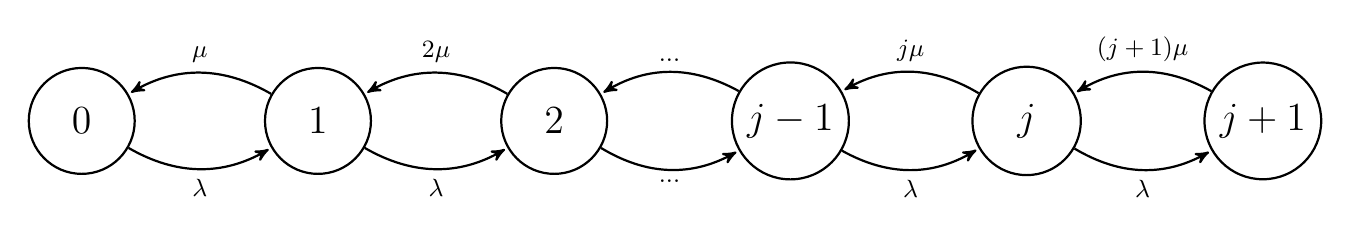
\begin{tikzpicture}[->,>=stealth',shorten >=1pt,auto,node distance=3cm,thick,main node/.style={circle,draw,font=\sffamily\Large\bfseries}]
  \node[main node] (1) {$~~0~~$};
  \node[main node] (2) [right of=1] {$~~1~~$};
  \node[main node] (3) [right of=2] {$~~2~~$};
  \node[main node] (4) [right of=3] {$j-1$};
  \node[main node] (5) [right of=4] {$~~j~~$};
  \node[main node] (6) [right of=5] {$j+1$};

  \path[every node/.style={font=\sffamily\small}]
    (1) edge [bend right=30] node[below]  {$\lambda$} (2)
    (2) edge [bend right=30] node[below]  {$\lambda$} (3)
    (3) edge [bend right=30] node[below]  {$...$} (4)
    (4) edge [bend right=30] node[below]  {$\lambda$} (5)
    (5) edge [bend right=30] node[below]  {$\lambda$} (6)
    (6) edge [bend right=30] node[above]  {$(j+1)\mu$} (5)
    (5) edge [bend right=30] node[above]  {$j\mu$} (4)
    (4) edge [bend right=30] node[above]  {$...$} (3)
    (3) edge [bend right=30] node[above]  {$2\mu$} (2)
    (2) edge [bend right=30] node[above]  {$\mu$} (1);
\end{tikzpicture}
\end{center}
And when $j\geq k$:
\begin{center}
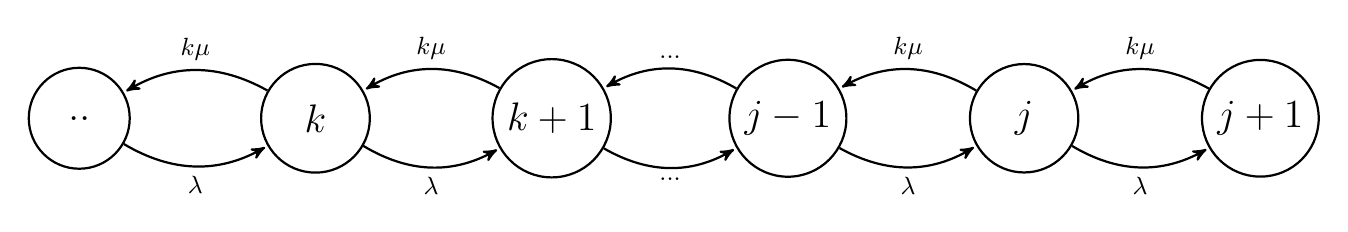
\begin{tikzpicture}[->,>=stealth',shorten >=1pt,auto,node distance=3cm,thick,main node/.style={circle,draw,font=\sffamily\Large\bfseries}]
  \node[main node] (1) {$~~..~~$};
  \node[main node] (2) [right of=1] {$~~k~~$};
  \node[main node] (3) [right of=2] {$k+1$};
  \node[main node] (4) [right of=3] {$j-1$};
  \node[main node] (5) [right of=4] {$~~j~~$};
  \node[main node] (6) [right of=5] {$j+1$};

  \path[every node/.style={font=\sffamily\small}]
    (1) edge [bend right=30] node[below]  {$\lambda$} (2)
    (2) edge [bend right=30] node[below]  {$\lambda$} (3)
    (3) edge [bend right=30] node[below]  {$...$} (4)
    (4) edge [bend right=30] node[below]  {$\lambda$} (5)
    (5) edge [bend right=30] node[below]  {$\lambda$} (6)
    (6) edge [bend right=30] node[above]  {$k\mu$} (5)
    (5) edge [bend right=30] node[above]  {$k\mu$} (4)
    (4) edge [bend right=30] node[above]  {$...$} (3)
    (3) edge [bend right=30] node[above]  {$k\mu$} (2)
    (2) edge [bend right=30] node[above]  {$k\mu$} (1);
\end{tikzpicture}
\end{center}
The balance equation is given by
\begin{equation}
  \begin{cases}
    (j\mu+\lambda)P_j = \lambda P_{j-1} + (j+1)\mu P_{j+1}& 0<j<k \\
    (k\mu+\lambda)P_j = \lambda P_{j-1} + k \mu P_{j+1}& j\geq k \\
    \lambda P_{0} = \mu P_1 \\
  \end{cases}
\end{equation}
Dente $\rho=\frac{\lambda}{\mu}$. Solve with \textit{Mathematica}, $\Rightarrow$
\begin{equation}
  \begin{cases}
  P_0 = \left(\sum_{i=1}^{k-1}\frac{(k\rho)^i}{i!}+\frac{(k\rho)^k}{k!}\frac{1}{1-\rho}\right)^{-1} \\
  P_j = P_0 \cdot \frac{(k\rho)^j}{j!},~~0<j<k \\
  P_j = P_0 \cdot \frac{k^k\rho^j}{k!},~~j\geq k \\
  \end{cases}
\end{equation}
\end{solution}


\noindent\rule{16cm}{0.4pt}
%\\\\\\\\\\\\\\\\\\\\\\\\\\\\\\\\\\\\\\\\\\\\\\\\\\\\\\\\\\\\\\\\\\\\\\\\\\\\\\\\\\\
%(5)
\begin{problem} 
\end{problem}
\begin{solution} ~
\begin{itemize}
  \item[$\cdot$] Denote $P_j=\mathbb{P}\left(\{\text{j men in system.}\}\right)$, $j\leq m$. Then there should be $m-j$ men finished before this time, and is about to rejoin the system.
  \item[$\cdot$] For these $m-j$ men, time to next rejoining is the minimum of $m-j$ Exp($\theta$)s, hence the transition rate is $(m-j)\theta$. This will make system goes $j\to j+1$. Similar analysis for $j-1\to j$ transition, this rate is $(m-j+1)\theta$
  \item[$\cdot$] The boundary condition is at node $P_0$ and $P_m$, which can be obtained by taking $j=1$ or $j=m-1$ in the graph below.
\end{itemize}
\begin{center}
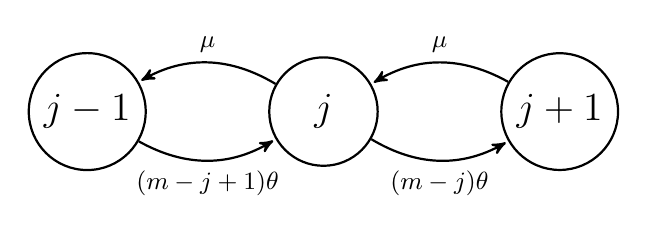
\begin{tikzpicture}[->,>=stealth',shorten >=1pt,auto,node distance=3cm,thick,main node/.style={circle,draw,font=\sffamily\Large\bfseries}]
  \node[main node] (1) {$j-1$};
  \node[main node] (2) [right of=1] {$~~j~~$};
  \node[main node] (3) [right of=2] {$j+1$};

  \path[every node/.style={font=\sffamily\small}]
    (1) edge [bend right=30] node[below]  {$(m-j+1)\theta$} (2)
    (2) edge [bend right=30] node[below]  {$(m-j)\theta$} (3)
    (3) edge [bend right=30] node[above]  {$\mu$} (2)
    (2) edge [bend right=30] node[above]  {$\mu$} (1);
\end{tikzpicture}
\end{center}
Hence we have BVP
\begin{equation}
  \begin{cases}
    (m-j+1)\theta P_{j-1} + \mu P_{j+1} = \mu P_j+ (m-j)\theta P_j & 0<j<m \\
    m\theta P_{0} = \mu P_1 \\
    \mu P_{m} = \theta P_{m-1} \\
  \end{cases}
\end{equation}
We postulate that $P_j$ is proportional to a weight function $w_j$, i.e. $P_j=\frac{w_j}{Z}$, $Z$ is normalizing factor. Solve via \textit{Mathematica}: 
\begin{equation}
  w_j = \frac{m!}{(m-j)!}\mu^{m-j}\theta^j;~~P_j = \frac{w_j}{\sum_{i=0}^m w_i}
\end{equation}
Check: 
\begin{equation}
  \begin{split}
    Z\times LHS &= (m-j+1)\theta w_{j-1} + \mu w_{j+1} = \frac{m!(m-j+1)}{(m-j+1)!}\mu^{m-j+1}\theta^{j} + \frac{m!}{(m-j-1)!}\mu^{m-j}\theta^{j+1} \\
    Z\times RHS &= \mu w_j+ (m-j)\theta w_j = \frac{m!}{(m-j)!}\mu^{m-j+1}\theta^j + \frac{m!(m-j)}{(m-j)!}\mu^{m-j}\theta^{j+1}
  \end{split}
\end{equation}
Check. Boundary also checks. Since stationary distribution is unique, this is exactly the solution.\\
(a)
\begin{equation}
  \lambda_a = \sum_{j=0}^m \lambda_j P_j = \sum_{j=0}^m (m-j)\theta P_j
\end{equation}
(b)
\begin{equation}
  W = \frac{L}{\lambda_a} = \frac{\sum_{j=0}^m j P_j}{\sum_{j=0}^m (m-j)\theta P_j}
\end{equation}
Where 
$$
P_j = \frac{\frac{m!}{(m-j)!}\mu^{m-j}\theta^j}{\sum_{i=1}^m \frac{m!}{(m-i)!}\mu^{m-i}\theta^i}
$$
\end{solution}

\noindent\rule{16cm}{0.4pt}
%\\\\\\\\\\\\\\\\\\\\\\\\\\\\\\\\\\\\\\\\\\\\\\\\\\\\\\\\\\\\\\\\\\\\\\\\\\\\\\\\\\\
\begin{problem} 
\end{problem}
\begin{solution}~
\begin{itemize}
  \item[$\cdot$] The arrival rate is always $\lambda$, departure is $2\mu$ at every $j\geq 2$. Graph is as below.
\end{itemize}
\begin{center}
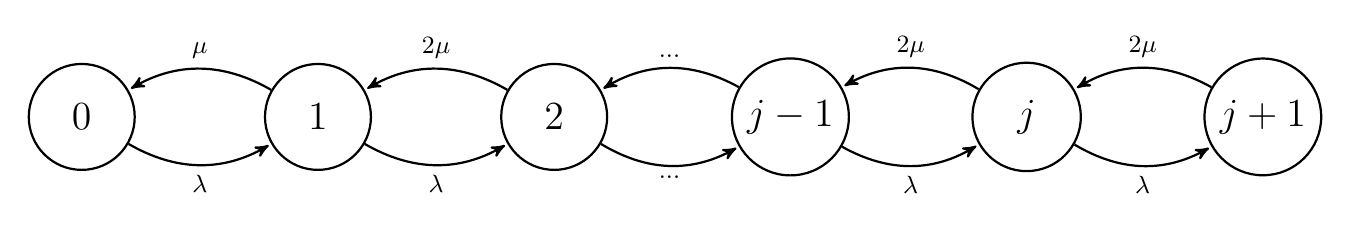
\begin{tikzpicture}[->,>=stealth',shorten >=1pt,auto,node distance=3cm,thick,main node/.style={circle,draw,font=\sffamily\Large\bfseries}]
  \node[main node] (1) {$~~0~~$};
  \node[main node] (2) [right of=1] {$~~1~~$};
  \node[main node] (3) [right of=2] {$~~2~~$};
  \node[main node] (4) [right of=3] {$j-1$};
  \node[main node] (5) [right of=4] {$~~j~~$};
  \node[main node] (6) [right of=5] {$j+1$};

  \path[every node/.style={font=\sffamily\small}]
    (1) edge [bend right=30] node[below]  {$\lambda$} (2)
    (2) edge [bend right=30] node[below]  {$\lambda$} (3)
    (3) edge [bend right=30] node[below]  {$...$} (4)
    (4) edge [bend right=30] node[below]  {$\lambda$} (5)
    (5) edge [bend right=30] node[below]  {$\lambda$} (6)
    (6) edge [bend right=30] node[above]  {$2\mu$} (5)
    (5) edge [bend right=30] node[above]  {$2\mu$} (4)
    (4) edge [bend right=30] node[above]  {$...$} (3)
    (3) edge [bend right=30] node[above]  {$2\mu$} (2)
    (2) edge [bend right=30] node[above]  {$\mu$} (1);
\end{tikzpicture}
\end{center}
\begin{equation}
  \begin{cases}
    \lambda P_{j-1} + 2\mu P_{j+1} = (2\mu + \lambda) P_j & j\geq 2 \\
    \lambda P_{0} = \mu P_1 \\
    \lambda P_{0} + 2\mu P_2 = (\mu + \lambda) P_1 \\
  \end{cases}
\end{equation}
(a) It turns out that
\begin{equation}
  P_0 = \frac{2\mu - \lambda}{2\mu + \lambda},~~~P_j = \frac{\lambda^j}{2^{j-1}\mu^j}P_0\text{ for }j\geq 1
\end{equation}
(b) 
\begin{equation}
  \begin{split}
    q(0,1) &= \lambda P_0 = \frac{\lambda(2\mu - \lambda)}{2\mu + \lambda} \\
    q(2,1) &= 2\mu P_2 = \frac{\lambda^2}{\mu}\cdot\frac{2\mu - \lambda}{2\mu + \lambda}
  \end{split}
\end{equation}
(c) It is clear that when $j\geq 2$ the stock clerk will be checking all the time. When $j=1$, the stock clerk can be also checking. This happens when the other clerk finishes before arrival at $j=2$, that is $S\leq T$ ($S$: service time, $T$: interarrival time). Hence
\begin{equation}
  \mathbb{P}\left(\{\text{stock clerk is checking, }j=1\}\right) = \mathbb{P}\left(S \leq T\right) P_2 = \frac{\lambda^2(2\mu - \lambda)}{2\mu(\mu+\lambda)(2\mu + \lambda)}
\end{equation}
Total proportion of time that he is checking is:
\begin{equation}
  \begin{split}
    p &= \mathbb{P}\left(\{\text{checking, }j=1\}\right) + \sum_{j\geq 2} P_j\\
    &= \frac{\lambda^2(2\mu - \lambda)}{2\mu(\mu+\lambda)(2\mu + \lambda)} + \frac{2 \lambda^2}{\mu(2\mu+\lambda)}
  \end{split}
\end{equation}
\end{solution}


\noindent\rule{16cm}{0.4pt}
%\\\\\\\\\\\\\\\\\\\\\\\\\\\\\\\\\\\\\\\\\\\\\\\\\\\\\\\\\\\\\\\\\\\\\\\\\\\\\\\\\\\
\begin{problem} 
\end{problem}
\begin{solution}~
\begin{itemize}
  \item[$\cdot$] There are only 4 states: system is full, only A or B is occupied, and 2 servers are both free. Denote these by $\{0, A, B, 2\}$. 
  \item[$\cdot$] New arrivals make the transition $B\to 2$ and $0\to A$ at state $B$ or $0$ when $A$ is free, with rate $\lambda=2$.
  \item[$\cdot$] Transition $B\to 0$ is made if $B$ finishes early then next arrival, w.p. $\frac{\lambda}{\mu_2+\lambda}$
  \item[$\cdot$] Transition $2\to A$ and $B\to 0$ is made with completion at $B$, rate is $\mu_B=2$. $2\to B$, and $A\to B$ is made with completion at $A$, rate is $\mu_A=4$.
\end{itemize}
\begin{center}
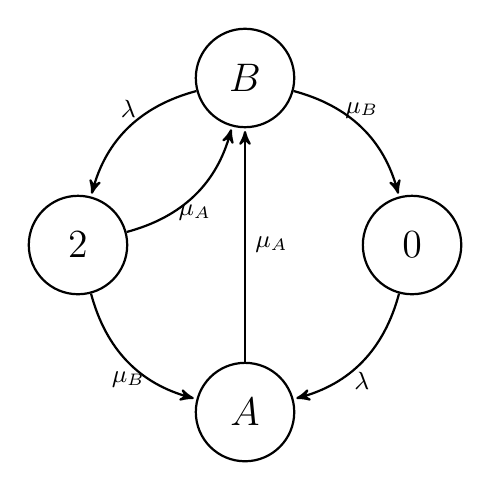
\begin{tikzpicture}[->,>=stealth',shorten >=1pt,auto,node distance=3cm,thick,main node/.style={circle,draw,minimum size=1.25cm,inner sep=0pt,font=\sffamily\Large\bfseries}]
  \node[main node] (1) {$2$};
  \node[main node] (2) [above right of=1] {$B$};
  \node[main node] (3) [below right of=1] {$A$};
  \node[main node] (4) [below right of=2] {$0$};

  \path[every node/.style={font=\sffamily\small}]
    (1) edge [bend right=30] node[below]  {$\mu_A$} (2)
    (1) edge [bend right=30] node[below]  {$\mu_B$} (3)
    (3) edge [right] node[right]  {$\mu_A$} (2)
    (2) edge [bend left=30] node[above]  {$\mu_B$} (4)
    (2) edge [bend right=30] node[above]  {$\lambda$} (1)
    (4) edge [bend left=30] node[below]  {$\lambda$} (3);
\end{tikzpicture}
\end{center}
\begin{equation}
  \begin{cases}
    \lambda P_0 = \mu_B P_B \\
    \mu_A P_A = \lambda P_0 + \mu_B P_2 \\
    (\mu_B + \lambda) P_B = \mu_A P_A + \mu_A P_2 \\
    (\mu_B + \mu_A) P_2 = \lambda P_B  \\
  \end{cases}
\end{equation}
(1) With $\lambda = 2$, $\mu_A = 4$, $\mu_B = 2$. It turns out that
\begin{equation}
  P_0 = \frac{1}{3},~~P_A = \frac{2}{9},~~P_B = \frac{1}{3},~~P_2 = \frac{1}{9}
\end{equation}
People can only enter at 0 or B. So define the events
\begin{equation}
  \begin{split}
    & E_0:=\{\text{enters the system at state [0]}\} \\
    & E:=\{\text{enters the system.}\}=E_0\cup E_B \\
    & S_B:=\{\text{receives service at B.}\}
  \end{split}
\end{equation}

\begin{equation}
  \mathbb{P}\left(E\right) = P_B + P_0 = \frac{2}{3}
\end{equation}
(b) When enter at state 0, there is nobody ahead of him that potentially prevent him from entering B. But if entering at state B, 
$$
\mathbb{P}\left(S_B|E_B\right)=\mathbb{P}\left(S_B \leq S_A\right) = \frac{\mu_B}{\mu_A+\mu_B} = \frac{1}{3}
$$
So
\begin{equation}
  \begin{split}
    \mathbb{P}\left(S_B|E\right) &= \mathbb{P}\left(S_B|E_B\right)\mathbb{P}\left(E_B|E\right) + \mathbb{P}\left(S_B|E_0\right)\mathbb{P}\left(E_0|E\right) \\
    &= \frac{\mu_B}{\mu_A+\mu_B} \times \frac{P_B}{P_0+P_B} + 1 \times \frac{P_0}{P_0+P_B} = \frac{2}{3}
  \end{split}
\end{equation}
(c) 
$$\mathbb{E}\left[N\right] = 0\cdot P_0 + 1\cdot(P_A+P_B)+2P_2 = \frac{7}{9}$$
(d) 
\begin{equation}
  \begin{split}
    \mathbb{E}\left[W|E\right] &= \mathbb{E}\left[W|E_B\right] \mathbb{P}\left(E_B|E\right) + \mathbb{E}\left[W|E_0\right] \mathbb{P}\left(E_0|E\right) \\
    &= \left(\mathbb{E}\left[S_A\right]+\mathbb{E}\left[S_B\right]\mathbb{P}\left(S_B|E_B\right)\right)\cdot\mathbb{P}\left(E_B|E\right)+ \mathbb{E}\left[S_A+S_B\right]\cdot\mathbb{P}\left(E_0|E\right)\\
    &= \left(\frac{1}{4}+\frac{1}{2}\cdot\frac{1}{3}\right)\cdot\frac{1}{2} + \left(\frac{1}{4}+\frac{1}{2}\right)\cdot\frac{1}{2} \\
    &= \frac{7}{12}
  \end{split}
\end{equation}
\end{solution}

\noindent\rule{16cm}{0.4pt}
%\\\\\\\\\\\\\\\\\\\\\\\\\\\\\\\\\\\\\\\\\\\\\\\\\\\\\\\\\\\\\\\\\\\\\\\\\\\\\\\\\\\
\begin{problem} 
\end{problem}
\begin{solution}~
\begin{itemize}
  \item[$\cdot$] Define the states as $\{0,1,...\}$ and $\{0^*,1^*,...\}$. $j$ represents there are $j$ men in the system, and $j^*$ means $j$ men and breaking down.
  \item[$\cdot$] For any state$^*$ that is not $0^*$, the rate of fixing up is $\beta$. And for any state that is not $0$, the rate of breaking down is $a$.
\end{itemize}
\begin{center}
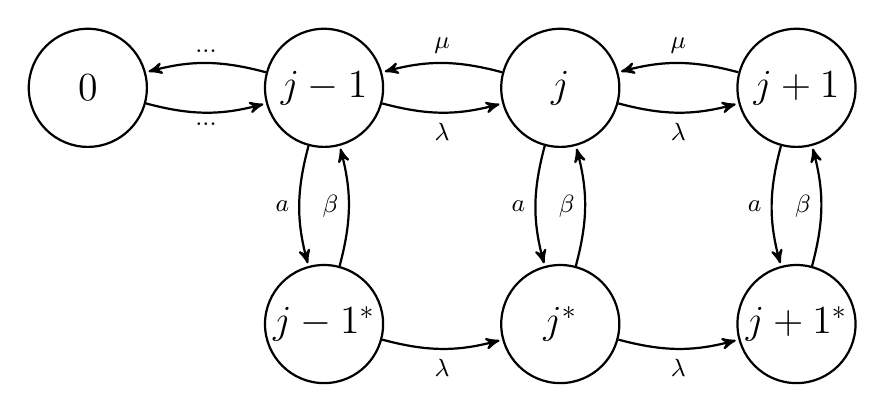
\begin{tikzpicture}[->,>=stealth',shorten >=1pt,auto,node distance=3cm,thick,main node/.style={minimum size=1.5cm,inner sep=0pt,circle,draw,font=\sffamily\Large\bfseries}]
  \node[main node] (1) {$j-1$};
  \node[main node] (2) [right of=1] {$~~j~~$};
  \node[main node] (3) [right of=2] {$j+1$};
  \node[main node] (4) [below of=1] {$j-1^*$};
  \node[main node] (5) [below of=2] {$~~j^*~~$};
  \node[main node] (6) [below of=3] {$j+1^*$};
  \node[main node] (7) [left of=1] {$0$};

  \path[every node/.style={font=\sffamily\small}]
    (1) edge [bend right=15] node[left]  {$a$} (4)
    (2) edge [bend right=15] node[left]  {$a$} (5)
    (3) edge [bend right=15] node[left]  {$a$} (6)
    (4) edge [bend right=15] node[left]  {$\beta$} (1)
    (5) edge [bend right=15] node[left]  {$\beta$} (2)
    (6) edge [bend right=15] node[left]  {$\beta$} (3)
    (1) edge [bend right=15] node[below]  {$\lambda$} (2)
    (2) edge [bend right=15] node[below]  {$\lambda$} (3)
    (7) edge [bend right=15] node[below]  {$...$} (1)
    (3) edge [bend right=15] node[above]  {$\mu$} (2)
    (2) edge [bend right=15] node[above]  {$\mu$} (1)
    (1) edge [bend right=15] node[above]  {$...$} (7)
    (4) edge [bend right=15] node[below]  {$\lambda$} (5)
    (5) edge [bend right=15] node[below]  {$\lambda$} (6);
\end{tikzpicture}
\end{center}
So the balance equation is given by
\begin{equation}
  \begin{cases}
    (\mu+\lambda+a)P_j = \lambda P_{j-1} + \mu P_{j+1} + \beta P_{j^*} & j\geq 1 \\
    (\lambda+\beta)P_{j^*} = \lambda P_{(j-1)^*} + a P_{j} & j^*\geq 2 \\
    \lambda P_0 = \mu P_{1} \\
    (\lambda+\beta)P_{1^*} =  a P_{1}
  \end{cases}
\end{equation}
So $\lambda_a =\lambda$.
\begin{equation}
  W = \frac{L}{\lambda_a} = \frac{\sum_{j\geq 0}j (P_j+P_{j^*})}{\lambda}
\end{equation}
\end{solution}


\noindent\rule{16cm}{0.4pt}
%\\\\\\\\\\\\\\\\\\\\\\\\\\\\\\\\\\\\\\\\\\\\\\\\\\\\\\\\\\\\\\\\\\\\\\\\\\\\\\\\\\\
\begin{problem} 
\end{problem}
\begin{solution}
\begin{itemize}
  \item[$\cdot$] If we regard time waiting in breakdown period as part of the ``service'', then the problem becomes a M/G/1. 
  \item[$\cdot$] Apply \textbf{Pollaczek-Khintchine}, we have
  $$
  W = \mathbb{E}\left[S\right] + \frac{\lambda \mathbb{E}\left[S^2\right]}{2(1- \lambda \mathbb{E}\left[S\right])}~~(\dag)
  $$
\end{itemize}
Then it suffices to calculate $\mathbb{E}\left[S\right]$ and $\mathbb{E}\left[S^2\right]$. \\
Define the followings
\begin{itemize}
  \item[$\cdot$] $S$ be the new ``service'' time. $\tilde{S}$ be the initial service time, $\tilde{S}\sim\text{Exp}(\mu)$. $A$ be the interarrivals of breakings, $A\sim\text{Exp}(a)$. $B$ be the time to fix up, $B\sim\text{Exp}(\beta)$. 
  \item[$\cdot$] $N$ the \# of breakdowns before finished. When a customer is serviced, $\mathbb{P}\left(\text{break down dose not occur}\right)=\mathbb{P}\left(\tilde{S}<A\right)=\frac{\mu}{\mu+a}$. We regard this as success probability, $N+1$ is therefore \# of trials until a success arises. Hence $N+1\sim$Geometric$(\frac{\mu}{\mu+a})$. We have
  $$
  \mathbb{E}\left[N\right] = \frac{\mu+a}{\mu},~~\mathrm{\mathbb{V}ar}\left[N\right] = \frac{a(\mu+a)}{\mu}
  $$ 
  \item[$\cdot$] $\{T_i\}$ be the sequence of time in service before another breakdown arises or the success. Then $T_i=\min\{\tilde{S}, A\}$. $T_i\sim\text{Exp}(\mu+a)$
\end{itemize}
The total ``service'' time is therefore
\begin{equation}
  \begin{split}
    &S = \sum_{i=1}^N (T_i + B_i) + T_{N+1} \\
    & \mathbb{E}\left[S|N\right] = \frac{N+1}{a+\mu} + \frac{N}{\beta}\\
    & \mathrm{\mathbb{V}ar}\left[S|N\right] =  \frac{N+1}{(a+\mu)^2} + \frac{N}{\beta^2}
  \end{split}
\end{equation}
Wald Identity $\Rightarrow$
\begin{equation}
  \mathbb{E}\left[S\right] = \mathbb{E}\left[\mathbb{E}\left[S|N\right]\right] = \frac{1}{\mu} + \frac{\mu+a}{\mu\beta} - \frac{1}{\beta} = \frac{1}{\mu} + \frac{a}{\mu \beta}
\end{equation}
And 
\begin{equation}
  \mathrm{\mathbb{V}ar}\left[S\right] = \left(\frac{1}{a+\mu} + \frac{1}{\beta}\right)^2 \frac{a(a+\mu)}{\mu^2}+\frac{1}{\mu(\mu+a)}+\frac{a}{\mu \beta^2}
\end{equation}
With these and $(\dag)$ we can calculate $W$, which is too lengthy to write.
\end{solution}

\noindent\rule{16cm}{0.4pt}
%\\\\\\\\\\\\\\\\\\\\\\\\\\\\\\\\\\\\\\\\\\\\\\\\\\\\\\\\\\\\\\\\\\\\\\\\\\\\\\\\\\\
\begin{problem} 
\end{problem}
\begin{solution} We have
\begin{itemize}
  \item[$\cdot$] External arrivals: $r_1= 5$, $r_2=10$, $r_3=15$.
  \item[$\cdot$] Service time $\mu_1 = 10$, $\mu_2=50$, $\mu_3=100$.
\end{itemize}
\begin{equation}
  \bm{P} = \begin{pmatrix}
    0 & \frac{1}{3} & \frac{1}{3} \\
    0 & 0 & 1 \\
    0 & \frac{1}{2} & 0 \\
  \end{pmatrix}
\end{equation}
And
\begin{equation}
  \lambda_j = r_j + \sum_{i=1}^3 \lambda_i P_{ij}
\end{equation}
(a) We solve out $\lambda_j$, and $\rho_j = \frac{\lambda_j}{\mu_j}$, $L_j=\frac{\rho_j}{1-\rho_j}=\frac{\lambda_j}{\mu_j - \lambda_j}$
\begin{equation}
  \begin{cases}
  \lambda_1 = 5 \\
  \lambda_2 = 40 \\
  \lambda_3 = \frac{170}{3}\\
  \end{cases}
  \Rightarrow 
  L = \sum_{j=1}^3\frac{\lambda_j}{\mu_j - \lambda_j} = 1+4+ \frac{17}{13}\approx 6.3
\end{equation}
(b)
\begin{equation}
  W = \frac{L}{\lambda_a} = \frac{L}{r_1+r_2+r_3} \approx 0.21
\end{equation}

\end{solution}

\noindent\rule{16cm}{0.4pt}
%\\\\\\\\\\\\\\\\\\\\\\\\\\\\\\\\\\\\\\\\\\\\\\\\\\\\\\\\\\\\\\\\\\\\\\\\\\\\\\\\\\\
\begin{problem} 
\end{problem}
\begin{solution} Denote $S$ the service time and $V$ the value of customer. The system is a M/G/1 queue. \\
$\mathbb{E}\left[V\right]=\frac{1}{2}$, $\mathrm{\mathbb{V}ar}\left[V\right]=\frac{1}{12}$, $\mathbb{E}\left[V^2\right]=\frac{1}{3}$.
\begin{equation}
  \begin{split}
    &\mathbb{E}\left[S\right] = \mathbb{E}\left[\mathbb{E}\left[S|V\right]\right] = \mathbb{E}\left[3+4V\right] = 5 \\
    &\mathbb{E}\left[S^2|V\right] = \mathbb{E}^2\left[S|V\right] + \mathrm{\mathbb{V}ar}\left[S|V\right] = 5+(3+4V)^2 \\
    &\mathbb{E}\left[S^2\right] = \mathbb{E}\left[\mathbb{E}\left[S^2|V\right]\right] = 5+9+24\cdot\frac{1}{2}+\frac{16}{3} = \frac{94}{3}
  \end{split}
\end{equation}
(a) Apply \textbf{Pollaczek-Khintchine}, we have
\begin{equation}
  \begin{split}
    W &= \mathbb{E}\left[S\right] + \frac{\lambda \mathbb{E}\left[S^2\right]}{2(1- \lambda \mathbb{E}\left[S\right])} \\
    &= \frac{94 \lambda/ 3}{2(1-5 \lambda)} +5
  \end{split}
\end{equation}
(b)
\begin{equation}
  W|\{V=x\} = \mathbb{E}\left[S|x\right] + W_Q = \frac{94 \lambda/ 3}{2(1-5 \lambda)} + 3+4x
\end{equation}
\end{solution}

\noindent\rule{16cm}{0.4pt}
%\\\\\\\\\\\\\\\\\\\\\\\\\\\\\\\\\\\\\\\\\\\\\\\\\\\\\\\\\\\\\\\\\\\\\\\\\\\\\\\\\\\
\begin{problem} 
\end{problem}
\begin{solution} (a) Denote $I$ the idle period, clearly $\mathbb{E}\left[I\right]=1/\lambda$. $P_0$ be long run proportion of time there is $0$ man in system. By results in the lecture, $1-P_0 = \lambda \mathbb{E}\left[S\right]$ and
\begin{equation}
  \begin{split}
    & P_0 = \frac{\mathbb{E}\left[I\right]}{\mathbb{E}\left[I\right]+\mathbb{E}\left[B\right]} = \frac{1/\lambda}{1/\lambda + \mathbb{E}\left[B\right]} \\
    \Rightarrow~~& \mathbb{E}\left[B\right] = \frac{1-P_0}{\lambda P_0} = \frac{\mathbb{E}\left[S\right]}{1- \lambda \mathbb{E}\left[S\right]}
  \end{split}
\end{equation}
By PASTA: $a_0:=\mathbb{P}\left(\{\text{Arrival observes 0 man in the queue.}\}\right)=P_0$. And hence
\begin{equation}
  \mathbb{E}\left[S\right] = a_0 \int_0^{\infty} \bar{G}_1(t)dt + (1-a_0)\int_0^{\infty} \bar{G}_2(t)dt
\end{equation}
Substitute $a_0$ with $P_0=1- \lambda \mathbb{E}\left[S\right]$, yields
\begin{equation}
  \mathbb{E}\left[S\right] = \frac{\int_0^{\infty} \bar{G}_1(t)dt}{1+\lambda \int_0^{\infty} \bar{G}_1(t)dt+ \lambda\int_0^{\infty} \bar{G}_2(t)dt}
\end{equation}
Therefore
\begin{equation}
  \mathbb{E}\left[B\right] = \frac{\int_0^{\infty} \bar{G}_1(t)dt}{1- \lambda\int_0^{\infty} \bar{G}_2(t)dt}
\end{equation}
(b) We have $a_0 = P_0 = 1/\mathbb{E}\left[C\right]$ $\Rightarrow$
\begin{equation}
  \mathbb{E}\left[C\right] = \frac{1}{1- \lambda \mathbb{E}\left[S\right]} = \frac{1+\int_0^{\infty} \bar{G}_1(t)dt-\int_0^{\infty} \bar{G}_2(t)dt}{1-\int_0^{\infty} \bar{G}_2(t)dt}
\end{equation}
\end{solution}

\noindent\rule{16cm}{0.4pt}
%\\\\\\\\\\\\\\\\\\\\\\\\\\\\\\\\\\\\\\\\\\\\\\\\\\\\\\\\\\\\\\\\\\\\\\\\\\\\\\\\\\\
\begin{problem} 
\end{problem}
\begin{solution} Define the followings
\begin{itemize}
  \item[$\cdot$] $T$ be the actual time in service, which has distribution $G$. 
  \item[$\cdot$] $N$ be the number of breakdowns. Since the service is continued after fixing ups, the time spent to fix server has noting to do with arrivals of breakdowns. Since the interarrival time of berakdowns is Exp($\alpha$), the number of breakdowns occurred up to time $t$ is a Poisson variable, i.e. $N\sim\text{Pois}(\alpha t)$.
  \item[$\cdot$] $R$ be the time spent fixing the server, has distribution $H$.
  \item[$\cdot$] $S$ be the total ``Service'' time including $\{R_i\}$s, we have
  $$S = \sum_{i=1}^N R_i + T$$
\end{itemize}
(a) Apply \textit{Pollaczek-Khintchine}, we have
$$
  W = \mathbb{E}\left[S\right] + \frac{\lambda \mathbb{E}\left[S^2\right]}{2(1- \lambda \mathbb{E}\left[S\right])}~~(\dag)
$$
Now it suffices to calculate $\mathbb{E}\left[S^2\right]$ and $\mathbb{E}\left[S\right]$.
\begin{equation}
  \begin{split}
    \mathbb{E}\left[S\right] &= \mathbb{E}\left[\mathbb{E}\left[S|T\right] \right]  \\
    &= \mathbb{E}\left[\alpha T \mathbb{E}\left[R\right]+\mathbb{E}\left[T\right]\right]\\
    &= \mathbb{E}\left[T\right]\left(\alpha \mathbb{E}\left[R\right]+1\right)
  \end{split}
\end{equation}
\begin{equation}
  \begin{split}
    \mathbb{E}\left[\mathbb{E}\left[S^2|T\right]\right] &=
    \mathbb{E}\left[\mathbb{E}\left[T^2 + 2T\sum_{i=1}^N R_i + \left(\sum_{i=i}^N R\right)^2 \middle|T\right] \right]\\
    & = \mathbb{E}\left[T^2 + 2T\cdot \alpha T \mathbb{E}\left[R\right] + \alpha T \mathbb{E}\left[R^2\right]+\alpha^2 T^2 \mathbb{E}^2\left[R\right]\right] \\
    &= \alpha \mathbb{E}\left[T\right] \mathbb{E}\left[R^2\right] + \mathbb{E}\left[T^2\right]\cdot 2 \alpha \mathbb{E}\left[R\right] + \mathbb{E}\left[T^2\right] + \mathbb{E}\left[T^2\right]\cdot \alpha^2 \mathbb{E}^2\left[R\right]\\
    &= \alpha \mathbb{E}\left[T\right] \mathbb{E}\left[R^2\right] + \mathbb{E}\left[T^2\right]\left(1+\alpha \mathbb{E}\left[R\right]\right)^2
  \end{split}
\end{equation}
Therefore
\begin{equation}
  W_Q = \frac{\alpha \mathbb{E}\left[T\right] \mathbb{E}\left[R^2\right] + \mathbb{E}\left[T^2\right]\left(1+\alpha \mathbb{E}\left[R\right]\right)^2}{2\left(1- \lambda\mathbb{E}\left[T\right]\left(\alpha \mathbb{E}\left[R\right]+1\right)\right)}~~(\dag)
\end{equation}
Where $T$ has known distribution $G$ and $R$ has known distribution $H$.\\
(b)
\begin{equation}
   L_Q = \lambda W_Q = \lambda\cdot(\dag)
 \end{equation} 
(c)
\begin{equation}
  W = W_Q + \mathbb{E}\left[S\right] = (\dag) + \mathbb{E}\left[T\right]\left(\alpha \mathbb{E}\left[R\right]+1\right)
\end{equation}
(d)
\begin{equation}
  L = \lambda W = \lambda \left((\dag)+\mathbb{E}\left[T\right]\left(\alpha \mathbb{E}\left[R\right]+1\right)\right)
\end{equation}
\end{solution}

\noindent\rule{16cm}{0.4pt}
%\\\\\\\\\\\\\\\\\\\\\\\\\\\\\\\\\\\\\\\\\\\\\\\\\\\\\\\\\\\\\\\\\\\\\\\\\\\\\\\\\\\
\begin{problem} 
\end{problem}
\begin{solution} (a) 
\begin{itemize}
  \item[$\cdot$] Assume service time $S$ has distribution $G$, WLOG assume $G$ has density $g(\cdot)$.
  \item[$\cdot$] $X_n$ be \# men in the queue at the departure of $n$th man. $Y_n$ be the \# of arrivals during $S_n$. Conditioning on $S_n$, $Y_n|\{S_n=t\}$ is Poisson with mean $\lambda t$. Hence we can compute
  \begin{equation}
    \begin{split}
      \mathbb{P}\left(Y_n=j\right) &= \int_0^{\infty} \mathbb{P}\left(Y_n=j|S_n=t\right)g(t)dt\\
      &= \int_0^{\infty} e^{-\lambda t}\frac{(\lambda t)^j}{j!}g(t)dt ~~(\dag)\\
    \end{split}
  \end{equation}
\end{itemize}
If $X_n>0$, $Y_{n+1}$ arrives in the $(n+1)$st service time, and when that guy departs, there is $X_{n+1}=X_n+Y_{n+1}-1$ (not counting himself) men in the system. \\
Otherwise if $X_n=0$, i.e. after $n$-th man departs, there is nobody in the queue. Then, $1$ man arrives and $S_{n+1}$ \textit{starts} on his arrrival, then $Y_{n+1}$ man arrives in $S_{n+1}$. Hence when he leaves, there are $Y_{n+1}$ men in the queue. We conclude that 
\begin{equation}
  X_{n+1} = \begin{cases}
  X_n + Y_{n+1}-1 & \text{if } X_n>0 \\
  Y_{n+1} & \text{if } X_n =0
  \end{cases}
\end{equation}
It is clear that $\{X_n\}$ is a markov chain, since it is determined by $X_{n}$ and $Y_{n+1}$, thus independent to any history before $n$-th departure. \\
(b) By the relation above and $(\dag)$
\begin{equation}
  \begin{split}
    P_{ij} &= \mathbb{P}\left(X_{n+1}=j|X_n = i\right)\\
    &= 
    \begin{cases}
    \mathbb{P}\left(i+Y_{n+1}-1 = j\right) & \text{if } i>0 \\
    \mathbb{P}\left(Y_{n+1}=j\right) & \text{if } i =0
    \end{cases} \\
    &= \begin{cases}
    \mathbb{P}\left(Y_{n+1} = j-i+1\right) & \text{if } i>0 \\
    \mathbb{P}\left(Y_{n+1}=j\right) & \text{if } i =0
    \end{cases} \\
    &= \begin{cases}
    0 & \text{if } i>0 \text{ and } j-i+1< 0\\
    \int_0^{\infty} e^{-\lambda t}\frac{(\lambda t)^{j-i+1}}{(j-i+1)!}g(t)dt & \text{if } i>0 \text{ and } j-i+1\geq 0\\
    \int_0^{\infty} e^{-\lambda t}\frac{(\lambda t)^j}{j!}g(t)dt & \text{if } i =0
    \end{cases} \\
  \end{split}
\end{equation}
We denote $p_j = \int_0^{\infty} e^{-\lambda t}\frac{(\lambda t)^j}{j!}g(t)dt$, then transition matrix is
\begin{equation}
  \bm{P} = \begin{pmatrix}
    p_0 & p_1 & p_2 & p_3 & ...  \\
    p_0 & p_1 & p_2 & p_3 & ...  \\
    0 & p_0 & p_1 & p_2 & ...  \\
    0 & 0 & p_0 & p_1 & ...  \\
    \vdots & \vdots & \vdots & \vdots & \ddots  \\
  \end{pmatrix}
\end{equation}
\end{solution}


\noindent\rule{16cm}{0.4pt}
%\\\\\\\\\\\\\\\\\\\\\\\\\\\\\\\\\\\\\\\\\\\\\\\\\\\\\\\\\\\\\\\\\\\\\\\\\\\\\\\\\\\
\begin{problem} 
\end{problem}
\begin{solution} ~
\begin{itemize}
  \item[$\cdot$] $X_n$ now is \# men in the system perceived by n-th arrival. Further define $Y_n$ is a counting of expoential events with rate $\mu$ durting the $n$-th interarrival time $T_n$, i.e. the \textbf{potential} \# of completion if there is sufficient customers in the queue.
  \item[$\cdot$] The queue is G/M/1, assume $T_n$ has known distribution $G$, and assume that $G$ has density $g(\cdot)$.
  \item[$\cdot$] Since the completion of service is Exp$(\mu)$, by same argument as Problem 14, conditioning on $T_n$, $Y_n\{T_n=t\}$ is Poisson variable with mean $\mu t$. So
  \begin{equation}
    \begin{split}
      \mathbb{P}\left(Y_n=j\right) &= \int_0^{\infty} \mathbb{P}\left(Y_n=j|T_n=t\right)g(t)dt\\
      &= \int_0^{\infty} e^{-\mu t}\frac{(\mu t)^j}{j!}g(t)dt ~~(\dag)\\
    \end{split}
  \end{equation}
  Denote this as $q_j$.
\end{itemize}
$X_n + 1$ is \# of men in system after the observer joins the queue, $Y_{n+1}$ is the \# of completion according to rate $\mu$, which is \textbf{not the actural} completion. When $X_n + 1 -Y_{n+1}<0$, implies the customer in system does not meet the server's capacity. Hence $n+1$-st arrival see nobody remains. $X_{n+1}=0$.\\
Otherwise, $X_{n+1}=X_n + 1 -Y_{n+1}$. Therefore
\begin{equation}
  X_{n+1} = \begin{cases}
  X_n + 1 -Y_{n+1} & \text{if } X_n + 1 -Y_{n+1}\leq 0 \\
  0 & \text{if } X_n + 1 -Y_{n+1} >0
  \end{cases}
\end{equation}
It is clear that $\{X_n\}$ is a markov chain, since it is determined by $X_{n}$ and $Y_{n+1}$, thus independent to any history before $n$-th arrival.\\
(b) 
\begin{equation}
  \begin{split}
    P_{ij} &= \mathbb{P}\left(X_{n+1}=j|X_n=i\right) = \\
    & = \begin{cases}
    0 & \text{if } j>0 \text{ and } i-j+1 < 0\\
    \mathbb{P}\left(Y_{n+1}=i-j+1\right) & \text{if } j>0 \text{ and } i-j+1\geq 0\\
    \mathbb{P}\left(Y_{n+1}\geq i+1\right) & \text{if } j=0
  \end{cases}
  \end{split}
\end{equation}
Hence the transition matrix is
\begin{equation}
  \bm{P} = \begin{pmatrix}
    \sum_{1}^{\infty}q_k & q_0 & 0 & 0 & ...  \\
    \sum_{2}^{\infty}q_k & q_1 & q_0 & 0 & ...  \\
    \sum_{3}^{\infty}q_k & q_2 & q_1 & q_0 & ...  \\
    \sum_{4}^{\infty}q_k & q_3 & q_2 & q_1 & ...  \\
    \vdots & \vdots & \vdots & \vdots & \ddots  \\
  \end{pmatrix}
\end{equation}
\end{solution}



\end{document}